\chapter{Overview of the LHCb upgrade}
\label{ref:lhcb-upgrade-overview}

% General changes
The run 2 of LHC has reached its conclusion at the end of 2018.
It has entered the second long shutdown (LS2) period since then.
During this period,
the upgrade on the LHC has enabled the accelerator to operate at
an unprecedented center of mass energy $\sqrt{s} = 13.6$~TeV with an
instantaneous luminosity of $2 \times 10^{33}$~cm$^{-2}$~s$^{-1}$
(for LHCb, a five-fold increase compared to run 2's number.
CMS and ATLAS operate at a luminosity 10 times as large)
\cite{CERN_news:2022,Piucci_2017}.
As of now\footnote{
    As a reminder, ``now'' refers to November 2022.
}, some of the LHCb subdetectors, for example the Upstream Tracker, are still
being upgraded.

% Motivate the LHCb upgrade
The upgraded LHC, however, poses unique problems for the LHCb experiment:
%%%%
With current hardware triggers\footnote{
    As discussed in \cref{ref:detector:trigger},
    the hardware triggers require the event to be above a certain $\pt / E_T$
    threshold.
},
to maintain a constant readout rate of 1~MHz,
the thresholds for \pt and $E_T$ have to increase,
which largely cancels the benefit of running at higher luminosity.
As shown in \cref{fig:l0-trigger-eff},
the \pt-based hadronic trigger yields are saturating even at run 2 luminosity
($4 \times 10^{32}$~cm$^{-2}$~s$^{-1}$).
%%%%
In addition, at $2 \times 10^{33}$~cm$^{-2}$~s$^{-1}$ a significant portion of
bunch crossings contains $b$ and $c$ signals.
With the current inclusive trigger scheme,
there will be too many ``signal-like'' events to write offline on storage
\cite{Albrecht_2014}.

\begin{figure}[!htb]
    \centering
    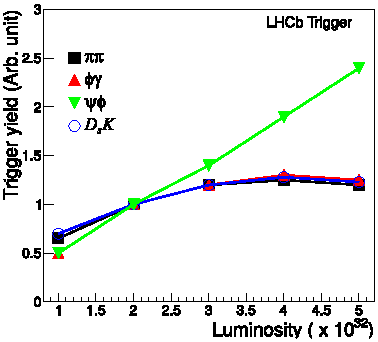
\includegraphics[width=0.5\textwidth]{./figs-lhcb-upgrade-overview/trigger_efficiency.pdf}
    \caption{
        L0 trigger yields normalized to that of run 1.
        The hadronic triggers are already saturated at run 2 luminosity.
        Taken from \cite{Albrecht_2014}.
    }
    \label{fig:l0-trigger-eff}
\end{figure}

To solve these problems, the detector readout rate is upgraded to 40~MHz,
the LHC bunch crossing rate,
without any hardware trigger.
By exposing all low-level variables to purely software-based high-level
triggers with more exclusive selection criteria,
events can be \emph{categorized} into exclusive signal decay modes more
efficiently with reasonable write throughputs.

Aside from the upgrade of the readout system and trigger scheme,
the tracking system is upgraded to provide better resolution and more
radiation tolerance to sustain the increased luminosity.
The subdetectors mainly used in L0 trigger, namely Muon station 1, SPD, and PS,
are removed altogether to reduce material in front of the calorimeters to
improve energy resolution.
The RICH1 detector which is responsible for PID is upgraded to reduce
occupancy\footnote{
    Defined as the fraction of detected photons over the total number of
    channels
    \cite{D_Ambrosio_2017}.
}
thus maintaining good PID efficiency.
The calorimeters (ECAL and HCAL) and the muon system will not undergo
substantial upgrades
\cite{Piucci_2017}.
The changes in the LHCb detector betwen run 1, 2 and run 3 are indicated
in \cref{fig:lhcb-detector-comparison}.

\begin{figure}[!htb]
    \centering
    \begin{subfigure}[t]{0.45\textwidth}
        \centering
        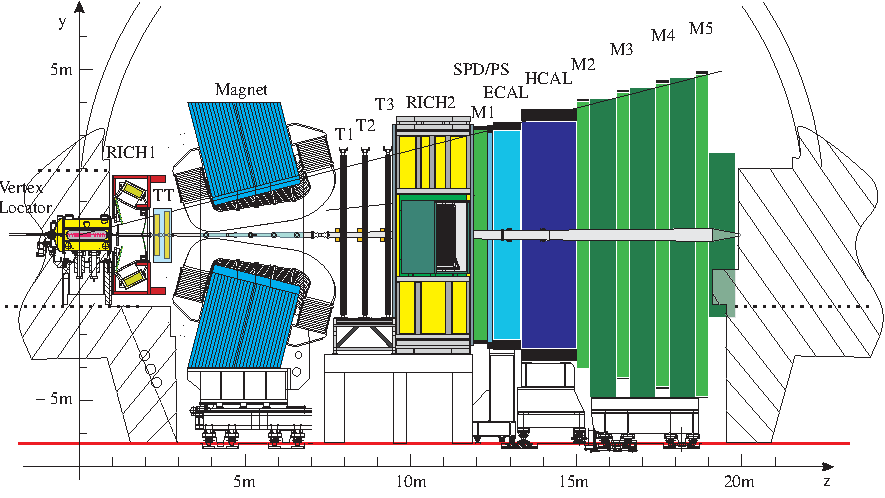
\includegraphics[width=\textwidth]{./figs-detector/lhcb_detector_view.pdf}
        \caption{The LHCb detector, run 1 and 2.}
    \end{subfigure}
    \hspace{12pt}
    %%%%
    \begin{subfigure}[t]{0.45\textwidth}
        \centering
        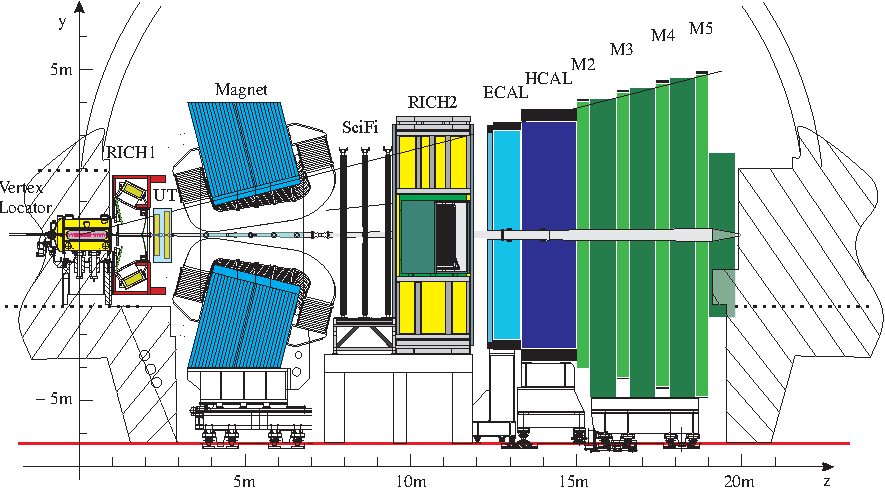
\includegraphics[width=\textwidth]{./figs-lhcb-upgrade-overview/lhcb_detector_view_run3.pdf}
        \caption{The upgraded LHCb detector in run 3.}
    \end{subfigure}

    \caption{
        The LHCb detector before (left) and after (right) LS2 upgrade.
        Note the upgrade on the tracking system:
        TT $\rightarrow$ UT, T-stations $\rightarrow$ SciFi;
        the removal of subdetectors relevant to L0 trigger only:
        The M1 muon station and SPD/PS have been removed.
    }
    \label{fig:lhcb-detector-comparison}
\end{figure}

The rest of the chapter provides an overview of the LHCb upgrade in LS2.
\cref{ref:lhcb-upgrade-overview:readout} describes the upgrade of the detector
readout system across all subdetectors.
Some subdetectors are undergoing upgrade to improve its performance, notably
the tracking and the PID system;
these will be discussed in \cref{ref:lhcb-upgrade-overview:tracking} and
\cref{ref:lhcb-upgrade-overview:tracking}, respectively.
Finally,
\cref{ref:lhcb-upgrade-overview:hlt}
provides an comparison of the trigger schemes between run 2 and run 3 and
explains how the detector upgrade solves the trigger bottleneck.


\section{Readout system}


\section{Trigger schemes in run 2 and run 3}
\label{ref:lhcb-upgrade-overview:trigger}


\section{Tracking system}
\label{ref:lhcb-upgrade-overview:tracking}

% Get a figure for old IT/OT combo vs. the new SciFi


\section{Particle identification system}
\label{ref:lhcb-upgrade-overview:tracking}


